\documentclass{article}

\usepackage{amsmath}
\usepackage{graphicx}
\usepackage{subcaption}
\usepackage{bigfoot}
\usepackage{hyperref}

\title{Project Overview}
\date{5 October 2018}
\author{
	ECE 388
	\\
	\\
	Team 4:
	\\
	Jacob Aubertine
	\\
	Mathieu Bolduc-Clayton
	\\
	Sal Fernandes
}

\begin{document}
	\pagenumbering{gobble}
	\maketitle
	\newpage
	\tableofcontents
	\newpage
	\pagenumbering{arabic}

	\section{Problem Statement}
	Problem statement goes here.

	% table
	\begin{table}[h!]
  		\begin{center}
    			\caption{Team member contributions.}
    			\label{tab:table1}
    			\begin{tabular}{r|r}
      				\textbf{Pulse width} & \textbf{Position (deg)} \\
				\hline
      				1 ms& -90 deg\\
      				1.25 ms & -45 deg\\
      				1.5 ms & 0 deg\\
      				1.75 ms & 45 deg\\
				2 ms& 90 deg\\
   			 \end{tabular}
  		\end{center}
	\end{table}

	\section{Description of subsystems}
	Describe subsystems here.
	
	\ref{fig:oscilloscope}.

	% figure
	\begin{figure}[h!]
		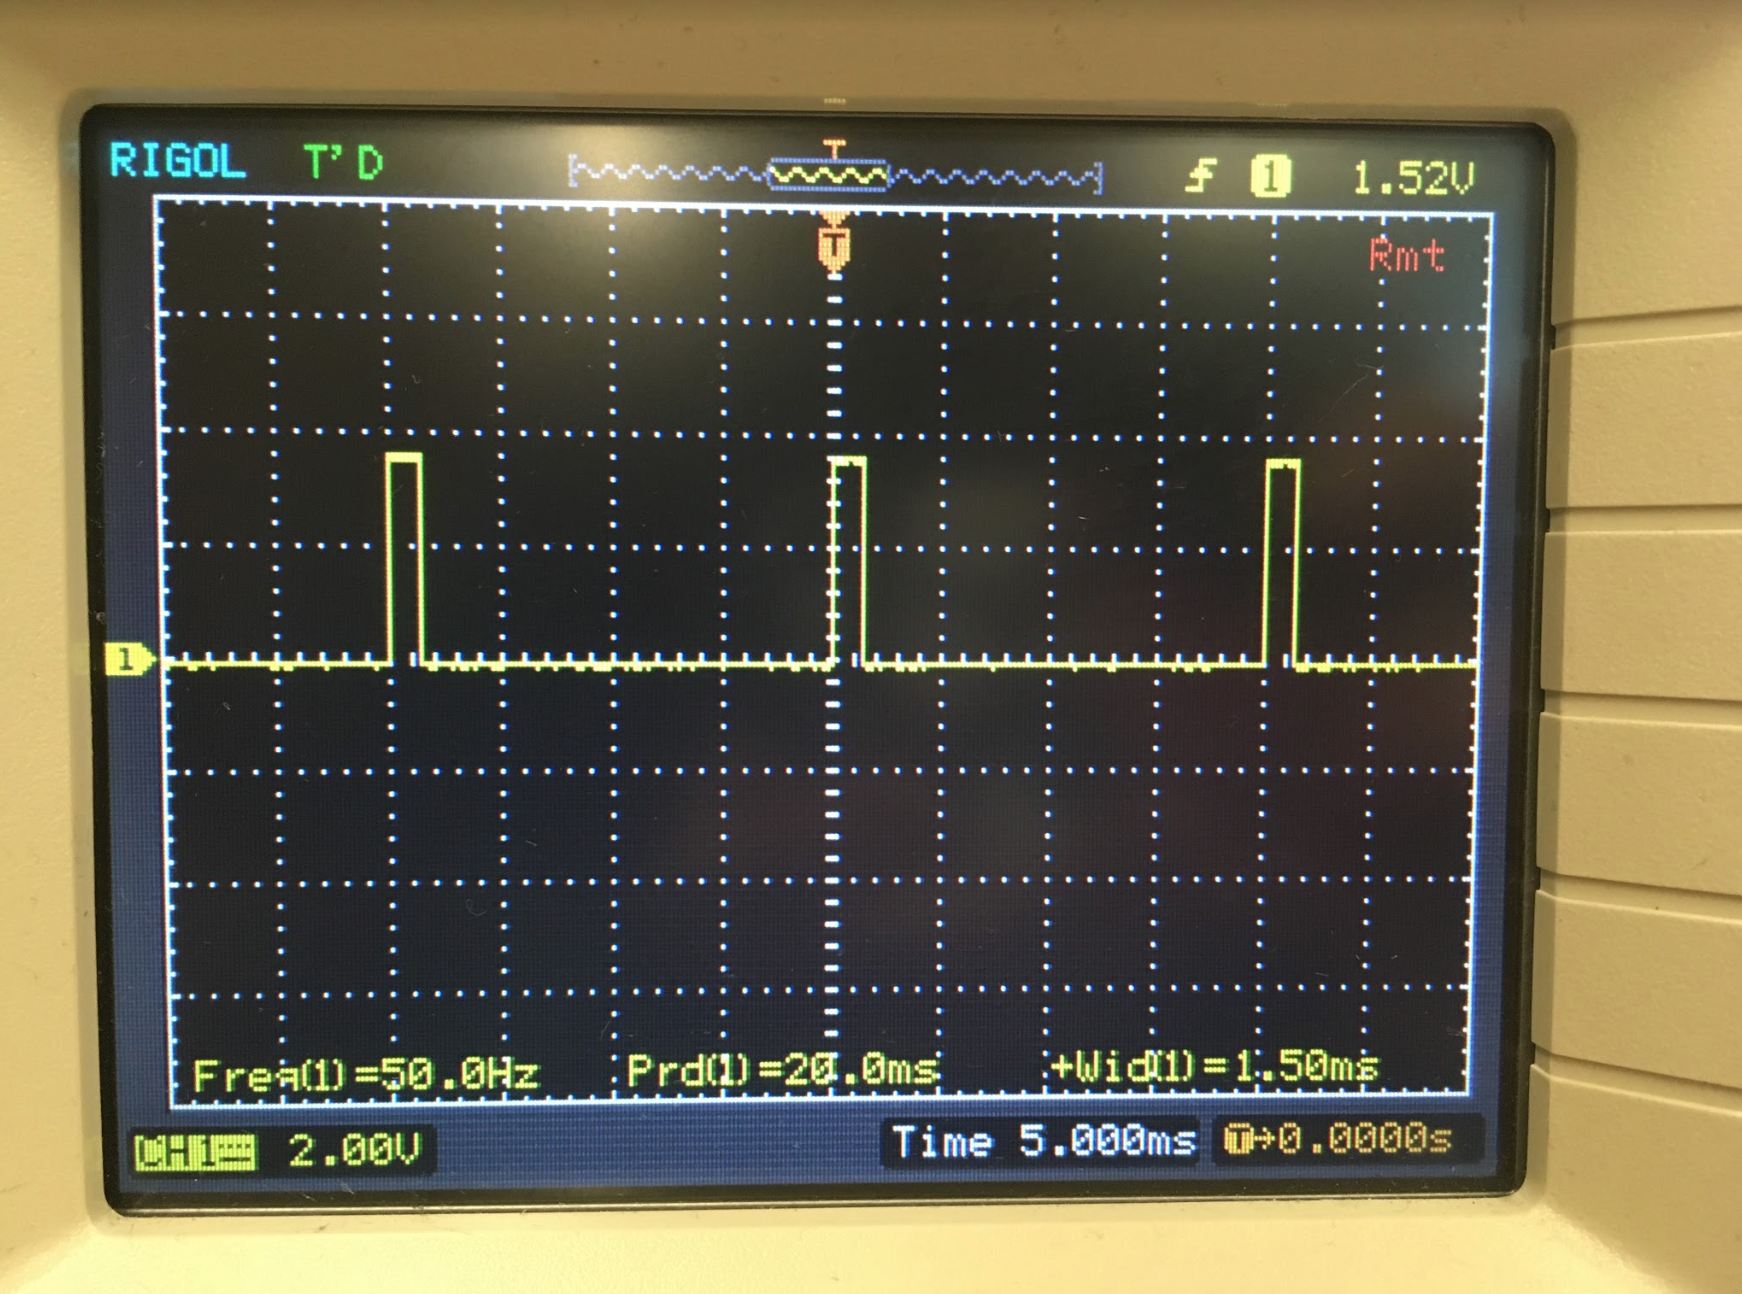
\includegraphics[width=\linewidth]{oscilloscope.png}
		\caption{Oscilloscope readings when connected to function generator.}
		\label{fig:oscilloscope}
	\end{figure}
	
	\section{Future test plans}
	Describe future test plans here.

\end{document}